
\section{Kết quả kiểm thử từng thành phần}
\label{sec:component_testing}

Trước khi tiến hành phân tích hiệu năng, các thử nghiệm chức năng được thực hiện để xác nhận rằng từng thành phần của hệ thống hoạt động đúng như thiết kế.  
Các log tiêu biểu và hình ảnh minh họa dưới đây cho thấy quá trình khởi tạo, kết nối, truyền dữ liệu định kỳ, phát hiện té ngã, xử lý cảnh báo và truyền hình ảnh.

\subsection{Module cảm biến đeo}
Module Quectel EC800K thuộc phần cứng cảm biến đeo được kiểm tra để xác nhận khả năng giao tiếp AT command, thiết lập kết nối 4G và thu nhận dữ liệu GPS.  

Quy trình kiểm thử bao gồm: khởi tạo UART, kiểm tra thông tin modem và SIM, đánh giá chất lượng sóng, cấu hình APN, kích hoạt PDP context, bật GPS và truy vấn tọa độ, sau đó tắt GPS và ngắt kết nối dữ liệu để tiết kiệm năng lượng.  

Kết quả cho thấy module hoạt động ổn định: thiết bị nhận diện đúng (EC800K), SIM sẵn sàng, tín hiệu mạnh (\texttt{+CSQ: 31,99}), kết nối dữ liệu thành công và thu được tọa độ GPS hợp lệ.

\textbf{Log tiêu biểu:}
\begin{minted}[fontsize=\footnotesize,breaklines]{text}
I (2329) SIM_4G: Received: Quectel EG800K
OK
I (5329) SIM_4G: Received: +CSQ: 31,99
OK
I (28339) SIM_4G: Received: +QIACT: 1,1,1,"9.204.251.200"
OK
I (34349) SIM_4G: Received: +QGPSLOC: 10.88862,106.77975
OK
\end{minted}

\textit{Kết luận:} Module 4G/GPS đã hoạt động đúng chức năng, đảm bảo hệ thống có thể gửi cảnh báo và thông tin định vị qua SMS/MQTT.

\subsection{Khởi tạo hệ thống và kết nối mạng}
Quá trình khởi tạo xác nhận rằng các module SIM4G-GPS, Wi-Fi và các tác vụ chính đều hoạt động bình thường, đảm bảo thiết bị sẵn sàng tham gia vào quá trình truyền thông và giám sát.

\begin{minted}[fontsize=\footnotesize,breaklines]{text}
I (9961) SIM4G_AT: Initializing SIM4G AT driver...
I (9981) SIM4G_AT: Successfully set APN to v-internet
I (10011) APP_MAIN: System initialization complete.
I (10021) APP_MAIN: Application started successfully
\end{minted}

\textit{Kết luận:} Hệ thống đã khởi tạo thành công, chứng minh nền tảng phần mềm và phần cứng được tích hợp ổn định.

\subsection{Kết nối MQTT và truyền dữ liệu}
Thiết bị ESP32 kết nối thành công với broker MQTT và thực hiện gửi bản tin định kỳ chứa thông tin định danh, trạng thái té ngã và dữ liệu GPS.  

\begin{minted}[fontsize=\footnotesize,breaklines]{text}
I (19961) USER_MQTT: MQTT_EVENT_CONNECTED
I (39991) JSON_WRAPPER: Created status payload:
{"device_id":"ESP32_DEV_76E48B","fall_detected":false,
 "latitude":0,"longitude":0,"has_gps_fix":false}
\end{minted}

\begin{figure}[H]
    \centering
    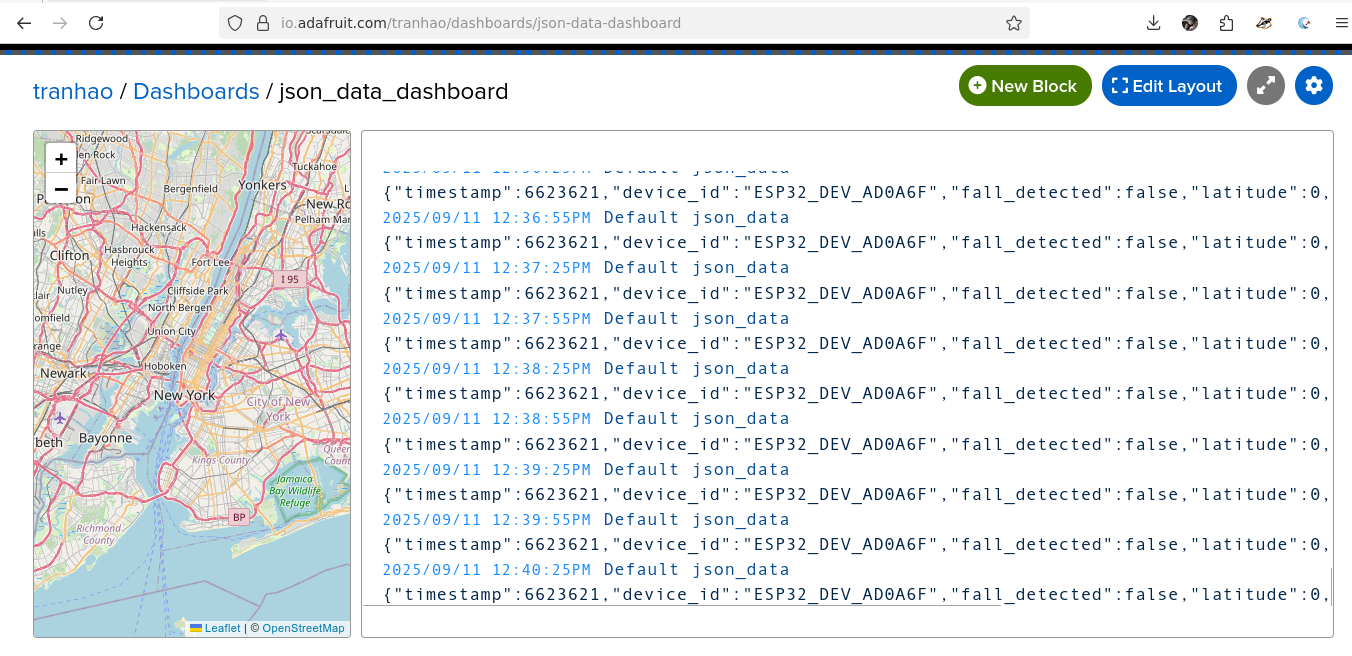
\includegraphics[width=0.8\textwidth]{figures/json_data_dashboard.png}
    \caption{Dashboard hiển thị bản tin MQTT từ thiết bị ESP32.}
    \label{fig:mqtt_dashboard}
\end{figure}

\textit{Kết luận:} Kết nối MQTT ổn định, đảm bảo thiết bị có thể truyền dữ liệu định kỳ tới hệ thống giám sát trung tâm.

\subsection{Phát hiện té ngã và xử lý cảnh báo}
Thuật toán phát hiện ghi nhận chuỗi trạng thái từ \texttt{LOW\_G} sang \texttt{HIGH\_G}, sau đó xác nhận va chạm và kích hoạt cảnh báo.  
Cảnh báo bao gồm gửi SMS, publish bản tin MQTT, đồng thời kích hoạt buzzer và LED cục bộ.  

\begin{minted}[fontsize=\footnotesize,breaklines]{text}
E (159131) FALL_LOGIC: FALL DETECTED! Accel: 0.99 g
I (159151) SIM4G_GPS: SMS request queued successfully
I (159191) SIM4G_GPS: MQTT alert published successfully.
I (159221) buzzer: Beeping for 8000 ms
I (159881) SIM4G_AT: SMS sent successfully.
I (175241) EVENT_HANDLER: Alert sequence completed.
\end{minted}

\begin{figure}[H]
    \centering
    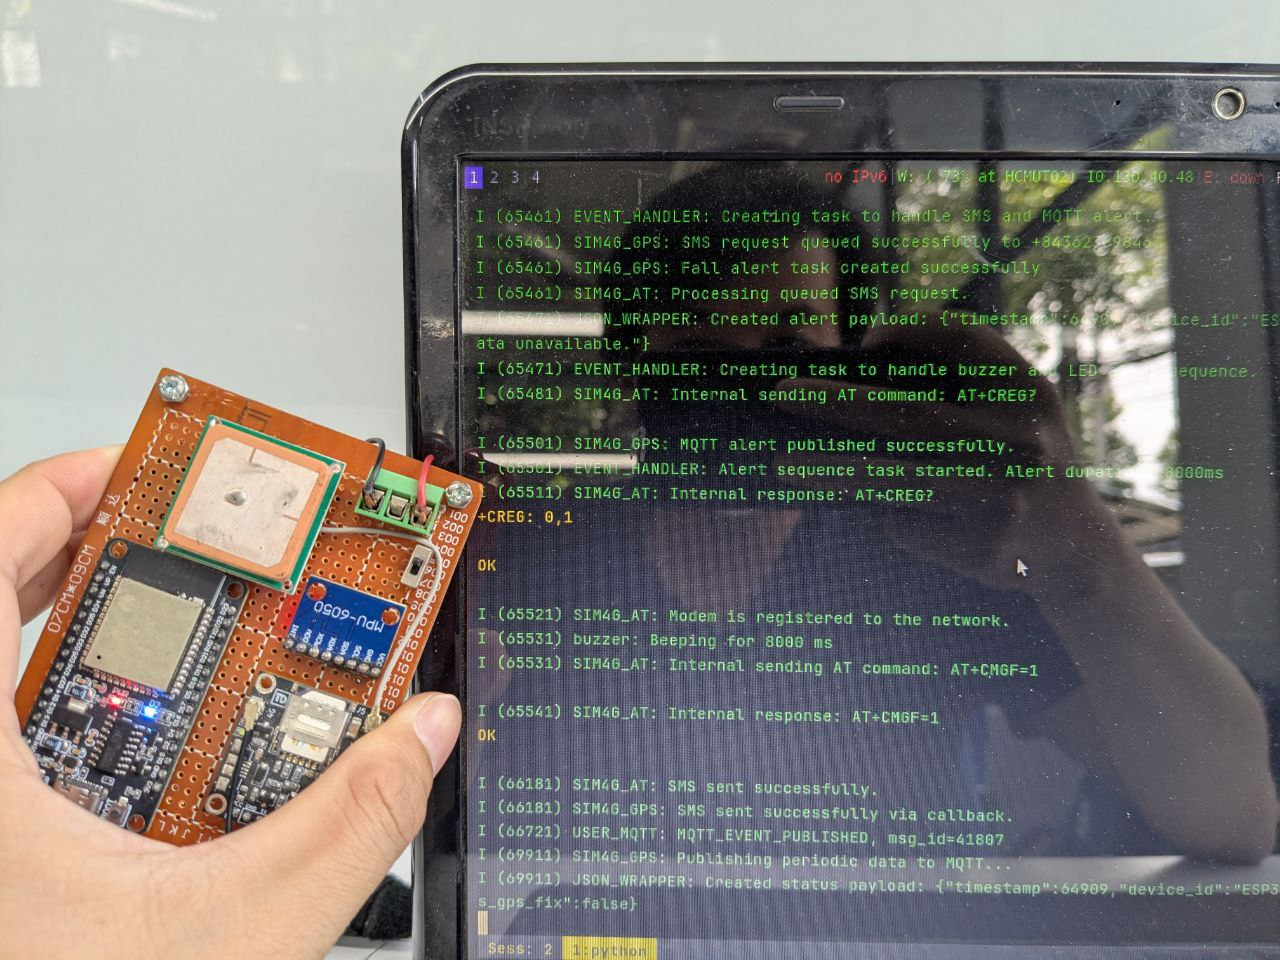
\includegraphics[width=0.8\textwidth]{figures/module1_real_log.jpg}
    \caption{Log thực tế của module cảm biến đeo khi phát hiện té ngã và kích hoạt cảnh báo.}
    \label{fig:module1_real_log}
\end{figure}

\textit{Kết luận:} Hệ thống phát hiện và xử lý cảnh báo té ngã thành công, kích hoạt đồng thời nhiều kênh cảnh báo.

\subsection{Module Camera và truyền hình ảnh}
Module ESP32-CAM được kiểm tra để xác nhận khả năng kết nối Wi-Fi và phát luồng hình ảnh qua HTTP.  
Kết quả log cho thấy camera được nhận diện đúng (OV5640), server HTTP đã khởi động và tốc độ khung hình trung bình dao động trong khoảng 3.5–5 FPS.
\begin{figure}[H]
    \centering
    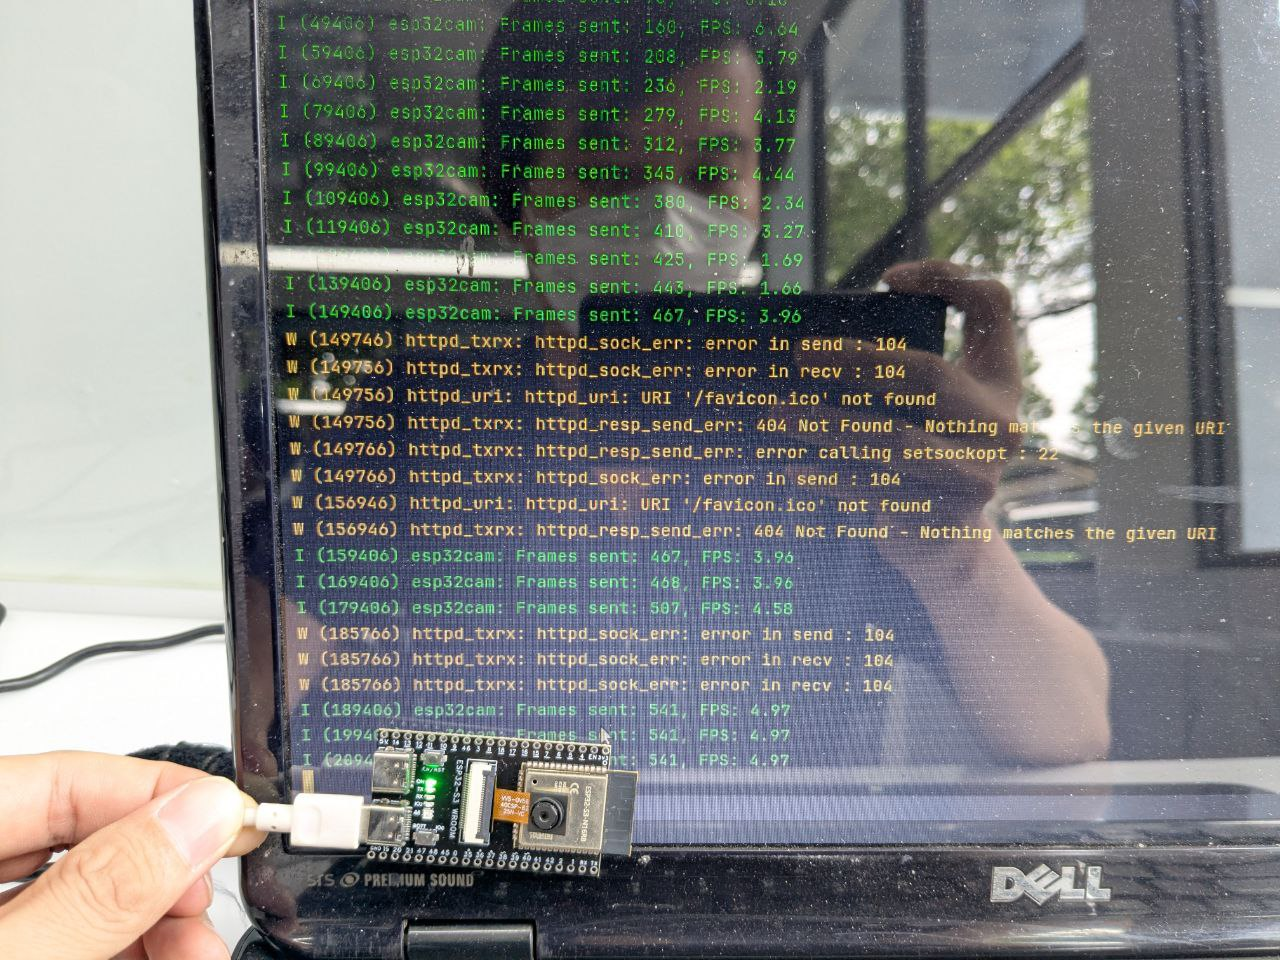
\includegraphics[width=0.8\textwidth]{figures/module2_real_log.jpg}
    \caption{Log thực tế của module esp-camera.}
    \label{fig:module2_real_log}
\end{figure}


\begin{minted}[fontsize=\footnotesize,breaklines]{text}
I (8936) esp32cam: Got IP: 10.110.87.85
I (9266) camera: Detected OV5640 camera
I (10006) esp32cam: HTTP server started
I (20006) esp32cam: Frames sent: 50, FPS: 5.87
I (40006) esp32cam: Frames sent: 146, FPS: 4.46
\end{minted}

\begin{figure}[H]
    \centering
    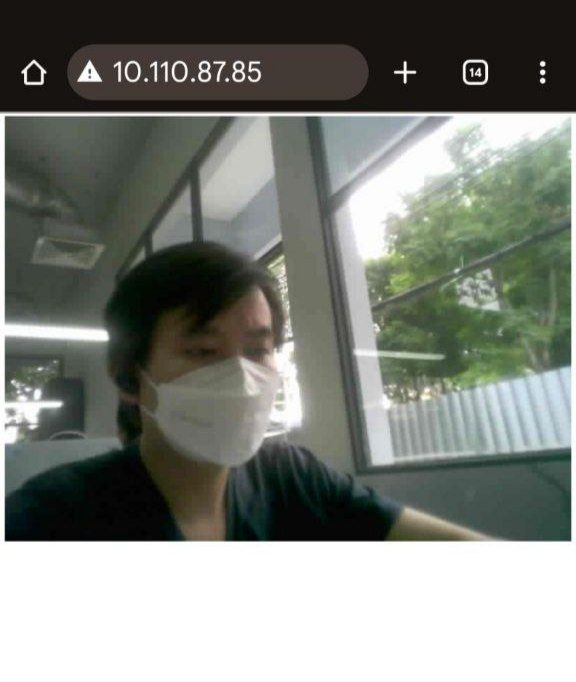
\includegraphics[width=0.8\textwidth]{figures/module2_stream_example.jpg}
    \caption{Luồng hình ảnh phát từ module ESP32-CAM qua HTTP.}
    \label{fig:camera_stream}
\end{figure}

\textit{Kết luận:} Module camera hoạt động ổn định, cho phép giám sát hình ảnh trực tiếp phục vụ xác minh sự kiện té ngã.

\subsection{Kiểm tra Xử lý nhận diện hình ảnh (Python)}
Module xử lý hình ảnh bằng Python nhận luồng video từ camera ESP32-CAM hoặc webcam, sau đó sử dụng TensorFlow Lite để phát hiện người và trích xuất các điểm khớp (skeleton) theo thời gian thực.  

Quy trình xử lý bao gồm:
\begin{itemize}
    \item Khởi tạo pipeline nhận luồng video từ camera.  
    \item Tiền xử lý khung hình (chuẩn hóa kích thước, màu sắc).  
    \item Chạy mô hình học máy TensorFlow Lite để phát hiện và trích xuất các điểm khớp của cơ thể người.  
    \item Vẽ skeleton trực quan trên khung hình để theo dõi trạng thái và chuyển động.  
\end{itemize}

Kết quả thực nghiệm cho thấy module hoạt động ổn định, xử lý khung hình theo thời gian thực với tốc độ trung bình 3--5 FPS.  
Hình~\ref{fig:python_skeleton} minh họa giao diện theo dõi người và skeleton được module xử lý hình ảnh tạo ra trong quá trình chạy thử nghiệm.

\begin{figure}[H]
    \centering
    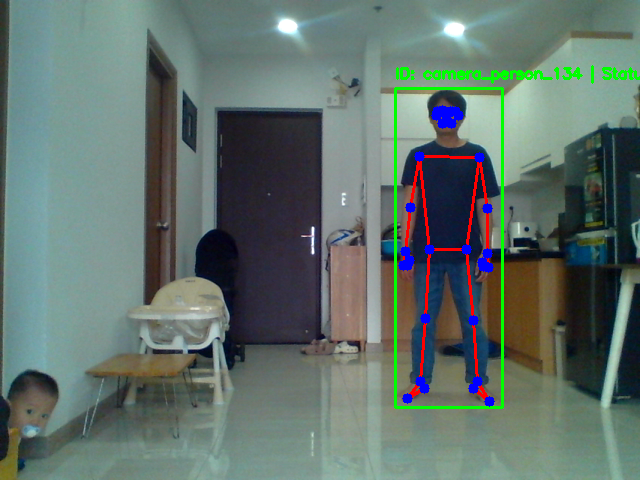
\includegraphics[width=0.85\textwidth]{figures/fall_detection_screen_shoot.png}
    \caption{Module Python xử lý hình ảnh: phát hiện người và vẽ skeleton theo thời gian thực.}
    \label{fig:python_skeleton}
\end{figure}


Module máy chủ xử lý được xây dựng bằng Python nhằm thực hiện các chức năng: thu nhận luồng dữ liệu từ camera, triển khai mô hình học sâu để dựng khung xương (skeleton), đồng thời tích hợp với hệ thống gửi cảnh báo qua MQTT và Telegram. Ngoài ra, module còn ghi log vào cơ sở dữ liệu SQLite và duy trì kết nối với Asterisk Management Interface (AMI).  

\begin{figure}[H]
    \centering
    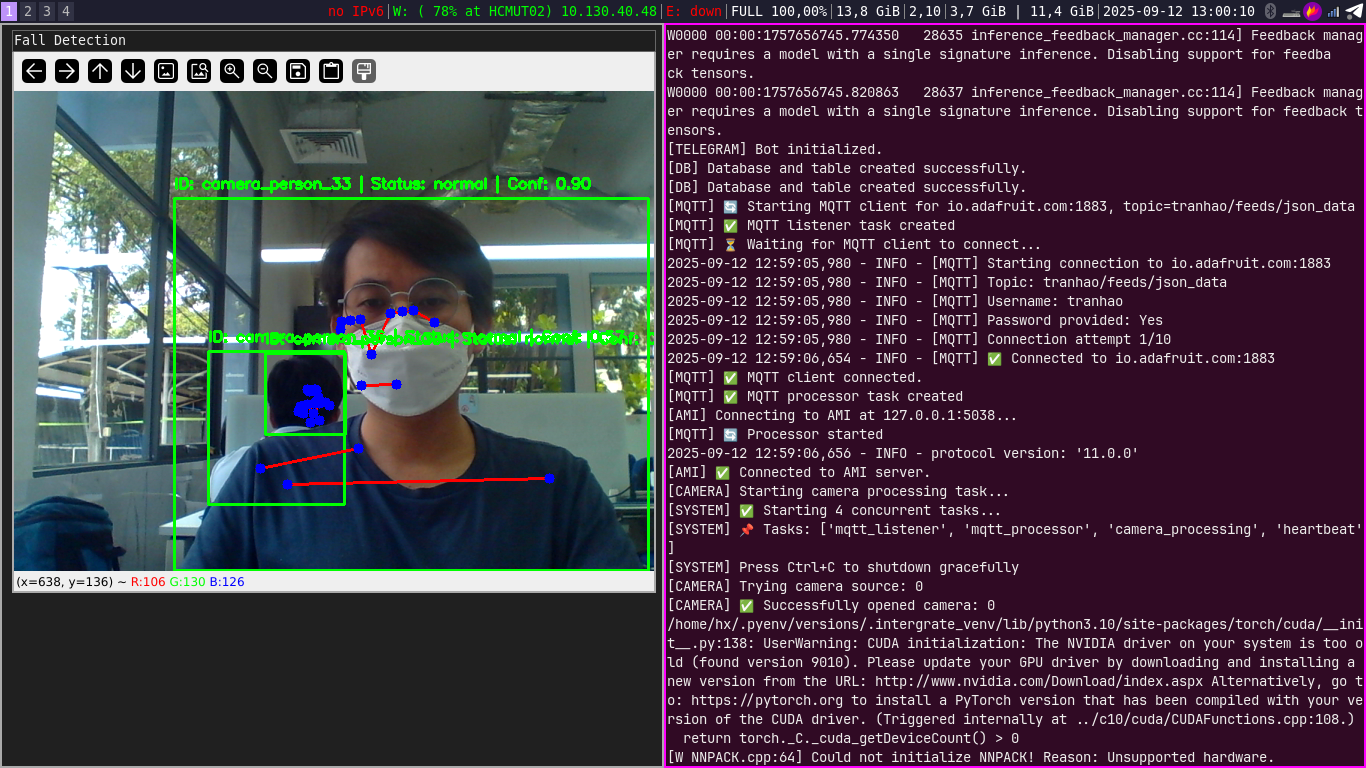
\includegraphics[width=0.8\textwidth]{figures/python_runing_log.png}
    \caption{Log thực nghiệm: Python xử lý ảnh và điều phối các tác vụ.}
    \label{fig:python_runing_log}
\end{figure}

\textbf{Kết luận:} Module Python đã hoạt động đúng chức năng, bảo đảm khả năng thu nhận dữ liệu camera, chạy nhận diện hình ảnh, đồng bộ dữ liệu qua MQTT, và kích hoạt các kênh cảnh báo. Hệ thống tuy có hạn chế về hỗ trợ CUDA (do phiên bản driver cũ) nhưng không ảnh hưởng đến quá trình thực thi trên CPU.

\subsection{Đánh giá thực nghiệm cảm biến mpu,gps và dữ liệu thu thập}
\subsubsection*{Quy trình thử nghiệm}
Để đánh giá hiệu quả hoạt động của hệ thống trong thực tế, quy trình thử nghiệm được tiến hành theo các bước:
\begin{enumerate}
    \item Nạp chương trình vào ESP32 bằng \texttt{idf.py flash monitor}.  
    \item Giả lập tình huống té ngã bằng cách lắc mạnh hoặc thả nhẹ thiết bị.  
    \item Quan sát log hệ thống để xác nhận sự kiện.  
    \item Kiểm tra tính năng gửi cảnh báo SMS với dữ liệu GPS.  
\end{enumerate}

\subsubsection*{Phân tích dữ liệu cảm biến}
Trong quá trình thử nghiệm, dữ liệu MPU6050 được thu thập cho hai trạng thái: \textbf{té ngã} và \textbf{bình thường}.  
Các bảng dưới đây trình bày dữ liệu đã ghi nhận.


\begin{table}[H]
\centering
\caption{Dữ liệu MPU6050 trong trạng thái té ngã}
\label{tab:fall_log_data}
\begin{tabularx}{\textwidth}{|c|>{\centering\arraybackslash}X|>{\centering\arraybackslash}X|>{\centering\arraybackslash}X|>{\centering\arraybackslash}X|>{\centering\arraybackslash}X|>{\centering\arraybackslash}X|}
\hline
\textbf{Time (ms)} & \textbf{Accel X (g)} & \textbf{Accel Y (g)} & \textbf{Accel Z (g)} & \textbf{Gyro X (dps)} & \textbf{Gyro Y (dps)} & \textbf{Gyro Z (dps)} \\
\hline
10338 & 0.06  & -0.12 & -1.00 & -22.50  & 47.18   & -77.85 \\
12338 & 0.20  & -0.09 & -0.96 & -79.74  & -64.79  & 22.34  \\
16338 & 0.10  & 0.02  & -1.19 & 23.37   & 14.82   & -4.84  \\
17338 & -0.25 & -0.13 & -0.82 & -42.96  & -8.53   & 18.43  \\
20338 & 0.18  & 0.07  & -1.02 & -50.80  & 32.41   & 15.31  \\
26338 & -1.56 & 1.06  & -2.00 & 168.47  & 250.13  & 116.60 \\
29338 & -2.00 & -1.69 & -1.29 & 250.13  & 250.13  & 38.65  \\
43338 & 0.33  & 0.07  & 0.23  & -157.85 & -61.94  & -188.73 \\
\hline
\end{tabularx}
\end{table}


\begin{table}[H]
\centering
\caption{Dữ liệu MPU6050 trong trạng thái bình thường}
\label{tab:normal_log_data}
\begin{tabularx}{\textwidth}{|c|X|X|X|X|X|X|}
\hline
\textbf{Time (ms)} & \textbf{Accel X (g)} & \textbf{Accel Y (g)} & \textbf{Accel Z (g)} & \textbf{Gyro X (dps)} & \textbf{Gyro Y (dps)} & \textbf{Gyro Z (dps)} \\
\hline
328  & -0.19 & -0.22 & -0.93 & 1.08 & -1.18 & 0.38 \\
1338 & -0.19 & -0.22 & -0.93 & 1.03 & -1.38 & 0.64 \\
2338 & -0.20 & -0.22 & -0.94 & 1.19 & -1.13 & 0.18 \\
3338 & -0.19 & -0.22 & -0.93 & 1.07 & -0.95 & 0.35 \\
4338 & -0.19 & -0.22 & -0.93 & 0.99 & -1.02 & -0.02 \\
5338 & -0.19 & -0.22 & -0.94 & 1.18 & -1.33 & 0.29 \\
6338 & -0.19 & -0.22 & -0.93 & 0.95 & -1.42 & 0.21 \\
\hline
\end{tabularx}
\end{table}

% Bảng so sánh
\begin{table}[H]
\centering
\caption{So sánh đặc trưng dữ liệu MPU6050 giữa trạng thái bình thường và té ngã}
\label{tab:mpu6050_new_comparison}
\begin{tabularx}{\textwidth}{|l|p{2.5cm}|p{2.5cm}|X|}
\hline
\textbf{Thông số} & \textbf{Bình thường} & \textbf{Té ngã} & \textbf{Nhận xét và ý nghĩa} \\
\hline
Biên độ Gyro (X,Y,Z) & $\pm 1.5$ dps & $\pm 250$ dps & Té ngã làm dao động góc tăng vọt, nhiều lần đạt cực trị giới hạn cảm biến. \\
\hline
Độ lớn Accel (XYZ) & $\approx -0.93$ g ổn định & dao động từ $-2.0$ g đến $+1.0$ g & Trạng thái bình thường chỉ phản ánh trọng lực, trong khi té ngã tạo biến thiên mạnh ở nhiều trục. \\
\hline
Độ lớn Gyro (Mag) & 1 -- 2 dps & 100 -- 400 dps & Rõ rệt sự khác biệt, té ngã gây xoay mạnh. \\
\hline
Độ lớn Accel (Mag) & 0.95 -- 0.97 g & 0.7 -- 2.0 g & Té ngã làm gia tốc tổng hợp vượt khỏi mức tĩnh, thể hiện xung lực va chạm. \\
\hline
\end{tabularx}
\end{table}

\begin{table}[H]
\centering
\caption{Dữ liệu vector (gia tốc và con quay hồi chuyển) theo ba trạng thái}
\label{tab:vector_data}
\begin{tabular}{|c|c|c|c|}
\hline
\textbf{Time (ms)} & \textbf{Accel\_Mag (g)} & \textbf{Gyro\_Mag (dps)} & \textbf{State} \\
\hline
328   & 0.99 & 1.66 & Normal \\
1338  & 1.01 & 1.77 & Normal \\
2338  & 1.02 & 1.70 & Normal \\
9338  & 1.05 & 5.80 & Fall \\
9438  & 1.27 & 5.77 & Fall \\
9538  & 1.21 & 5.90 & Fall \\
10338 & 1.00 & 0.25 & Post-Fall \\
11338 & 1.02 & 0.09 & Post-Fall \\
12338 & 1.01 & 0.15 & Post-Fall \\
\hline
\end{tabular}
\end{table}

\begin{figure}[H]
    \centering
    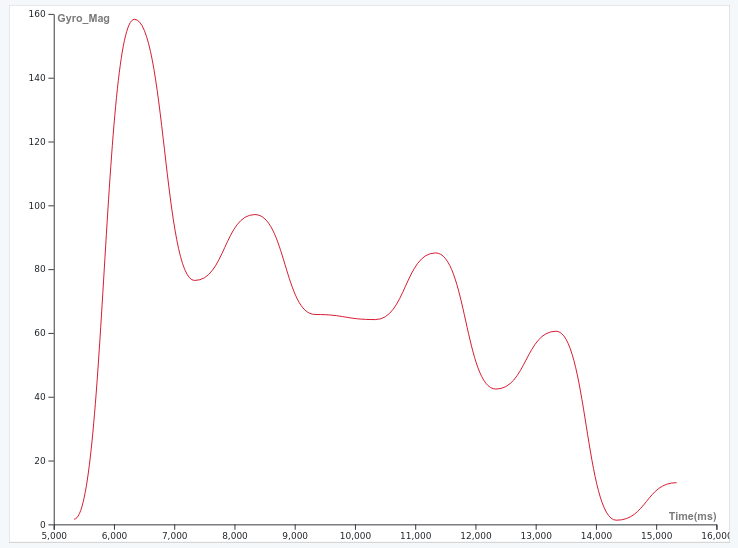
\includegraphics[width=0.95\linewidth]{figures/gyro_time.png}
    \caption{Biến thiên magnitude của gia tốc góc (Gyro\_Mag) theo thời gian.}
    \label{fig:gyro_time}
\end{figure}

\paragraph{Miêu tả và phân tích (Gyro theo thời gian).}
Đồ thị \ref{fig:gyro_time} biểu diễn biến thiên của đại lượng \texttt{Gyro\_Mag} (magnitude của vector con quay hồi chuyển) theo mốc thời gian thử nghiệm. Đồ thị thể hiện rõ ba pha hoạt động: 
\begin{itemize}
  \item \textbf{Bình thường (Normal):} \texttt{Gyro\_Mag} dao động rất nhỏ quanh giá trị nền (thường $\lesssim 2$ dps), biểu thị chuyển động góc nhẹ hoặc ổn định khi đeo thiết bị.
  \item \textbf{Sự kiện té ngã (Fall):} tại thời điểm xảy ra té, xuất hiện đỉnh đột biến lớn (thường tăng lên hàng chục đến hàng trăm dps). Các đỉnh này là đặc trưng nhận diện sự xoay mạnh và va chạm trong pha té.
  \item \textbf{Hậu té (Post-Fall):} sau đỉnh, \texttt{Gyro\_Mag} giảm nhanh về mức nền hoặc gần không, thể hiện trạng thái nằm yên và thiếu chuyển động góc.
\end{itemize}

Những quan sát quan trọng rút ra từ đồ thị:
\begin{enumerate}
  \item Biên độ đỉnh \texttt{Gyro\_Mag} trong pha \textit{Fall} lớn hơn nhiều so với dao động nền — hiệu quả để làm ngưỡng phân loại (ví dụ threshold tạm ứng: $>20$--$50$ dps tùy thực nghiệm).
  \item Hình thái thời gian của đỉnh (rise time và decay) cho phép phân biệt giữa cú va chạm thực sự và nhiễu ngắn (spike): cú té thật thường có đỉnh rộng hơn và kèm biến động phụ ở các trục.
\end{enumerate}

\vspace{6pt}

\begin{figure}[H]
    \centering
    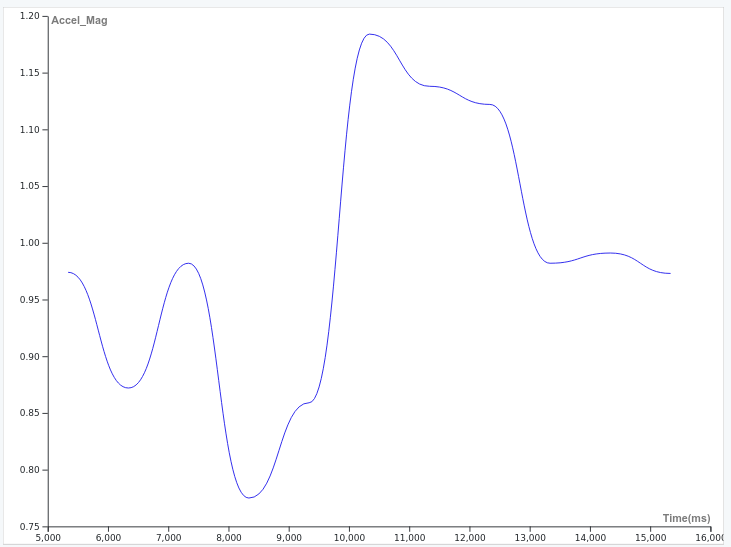
\includegraphics[width=0.95\linewidth]{figures/accel_time.png}
    \caption{Biến thiên magnitude của gia tốc (Accel\_Mag) theo thời gian.}
    \label{fig:accel_time}
\end{figure}

\paragraph{Miêu tả và phân tích (Accel theo thời gian).}
Đồ thị \ref{fig:accel_time} trình bày biến thiên \texttt{Accel\_Mag} (magnitude của vector gia tốc) theo cùng mốc thời gian. Diễn biến cũng chia làm ba pha tương tự:
\begin{itemize}
  \item \textbf{Bình thường (Normal):} \texttt{Accel\_Mag} nằm gần 1\,g (do trọng lực), dao động nhẹ quanh giá trị này khi người vận động nhẹ.
  \item \textbf{Sự kiện té ngã (Fall):} \texttt{Accel\_Mag} xuất hiện các xung hoặc thay đổi đột ngột, có thể vượt hoặc giảm mạnh so với 1\,g (tùy hướng va chạm), đặc biệt khi có va chạm mạnh xung lực tổng hợp có xu hướng lớn hơn 1\,g đáng kể.
  \item \textbf{Hậu té (Post-Fall):} \texttt{Accel\_Mag} trở về gần 1\,g nhưng với phân bố vector (các thành phần X/Y/Z) có thể đổi hướng so với trạng thái trước té (chỉ ra tư thế nằm).
\end{itemize}

\begin{enumerate}
  \item Sự tăng/giảm đột ngột của \texttt{Accel\_Mag} là chỉ báo trực tiếp của xung lực trong sự kiện té; phối hợp với \texttt{Gyro\_Mag} giúp loại bỏ nhiễu giả   \item Dao động nền quanh 1\,g cho phép hiệu chuẩn nhanh: mọi giá trị lệch bền khỏi 1\,g trong một khoảng thời gian ngắn.
\end{enumerate}

\textit{Kết luận:} Dữ liệu cảm biến cho thấy sự khác biệt rõ rệt giữa hai trạng thái. Đặc biệt, \textbf{Accel Mag} và \textbf{Gyro Mag} là chỉ báo hiệu quả để phát hiện té ngã, cung cấp cơ sở thực nghiệm cho việc tinh chỉnh ngưỡng phát hiện và giảm thiểu cảnh báo sai.

\begin{table}[H]
\centering
\caption{Bảng kết quả thu được từ log test của mô-đun 4G/GPS}
\label{tab:gps_data}
\begin{tabular}{|c|c|c|c|c|c|c|}
\hline
\textbf{Time (UTC)} & \textbf{Latitude} & \textbf{Longitude} & \textbf{Altitude (m)} & \textbf{Fix Mode} & \textbf{Date} & \textbf{Satellites} \\
\hline
132517.00 & 1053.3115N & 10646.7839E & 5.07 & 3 & 240425 & 07 \\
132517.00 & 1053.3115N & 10646.7839E & 5.07 & 3 & 240425 & 07 \\
132540.00 & 1053.3117N & 10646.7840E & 5.05 & 3 & 240425 & 07 \\
132540.00 & 1053.3117N & 10646.7840E & 5.05 & 3 & 240425 & 07 \\
132627.00 & 1053.3107N & 10646.7839E & 5.02 & 3 & 240425 & 07 \\
132627.00 & 1053.3107N & 10646.7839E & 5.02 & 3 & 240425 & 07 \\
\hline
\end{tabular}
\end{table}
% Bảng dữ liệu té ngã
% Bảng dữ liệu bình thường
% Bảng dữ liệu GPS



\begin{table}[H]
\centering
\caption{Phân tích và giải thích dữ liệu GPS thu được}
\label{tab:gps_analysis}
\renewcommand{\arraystretch}{1.3}
\begin{tabularx}{\textwidth}{|p{3cm}|p{3cm}|X|}
\hline
\textbf{Trường dữ liệu} & \textbf{Giá trị điển hình} & \textbf{Giải thích và ý nghĩa} \\
\hline
Thời gian (UTC) & 132517.00 -- 132627.00 & Dữ liệu được ghi nhận liên tục trong khoảng 1 phút; cho thấy tín hiệu GPS ổn định và không bị gián đoạn. \\
\hline
Vĩ độ (Latitude) & 10°53.3115'N & Vị trí xác định chính xác đến phần giây thập phân, phù hợp với khu vực thử nghiệm thực tế. \\
\hline
Kinh độ (Longitude) & 106°46.7839'E & Giá trị duy trì ổn định qua nhiều lần đo; chứng tỏ tín hiệu ít nhiễu và đáng tin cậy. \\
\hline
Độ cao (Altitude) & $\approx 5$ m & Độ cao phản ánh đúng địa hình khu vực thử nghiệm, dao động rất nhỏ (±0.05 m). \\
\hline
Chế độ định vị (Fix Mode) & 3 & Chế độ định vị 3D, đảm bảo độ chính xác cao khi xác định cả vĩ độ, kinh độ và độ cao. \\
\hline
Ngày (Date) & 24/04/2025 & Thời điểm dữ liệu được ghi nhận, khớp với lịch trình thử nghiệm. \\
\hline
Số vệ tinh (Satellites) & 07 & Số vệ tinh thu được đủ lớn để đảm bảo tín hiệu ổn định, độ tin cậy cao trong định vị. \\
\hline
\end{tabularx}
\end{table}
\subsection{Kết quả thử nghiệm chức năng gọi và nhắn tin cảnh báo qua Asterisk AMI}
\label{subsec:ast_call_sms_test}

Để kiểm chứng khả năng kích hoạt cảnh báo tự động qua tổng đài Asterisk, hệ thống đã được cấu hình thực hiện đồng thời cuộc gọi và gửi tin nhắn SMS đến ba extension (\texttt{6001}, \texttt{6002}, \texttt{6003}). Kết quả log thử nghiệm được thể hiện trong Hình~\ref{fig:ast_call_sms_test}.

Như quan sát trên log, quá trình kết nối tới Asterisk AMI được thực hiện thành công và hệ thống đã gửi tin nhắn đến các extension. Tin nhắn SMS tới \texttt{6001} và \texttt{6002} được gửi thành công, trong khi SMS tới \texttt{6003} gặp lỗi truyền tải. Ngoài ra, các dòng báo lỗi cuối cùng liên quan tới thao tác gọi điện xuất hiện do hệ thống chỉ kích hoạt cuộc gọi báo động mà không có nội dung thoại kèm theo. Việc này dẫn đến ngoại lệ \texttt{'list' object has no attribute 'get'}, nhưng không ảnh hưởng tới cơ chế gửi cảnh báo chính.

\begin{figure}[H]
    \centering
    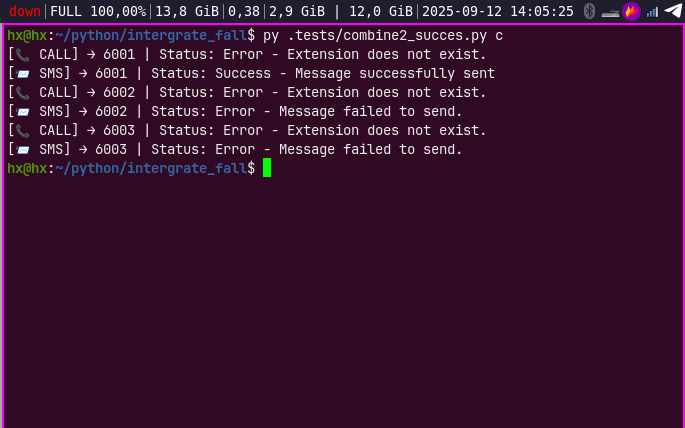
\includegraphics[width=0.95\linewidth]{figures/ast_call_sms_test.png}
    \caption{Kết quả thử nghiệm chức năng gọi và nhắn tin cảnh báo qua Asterisk AMI}
    \label{fig:ast_call_sms_test}
\end{figure}

\textit{Kết luận:}Kết quả thử nghiệm cho thấy hệ thống có thể gửi cảnh báo qua cuộc gọi và SMS thành công tới các extension, ngoại trừ một số lỗi ngoại lệ khi gọi điện do không có nội dung thoại, nhưng điều này không ảnh hưởng đến chức năng cảnh báo chính, chứng minh khả năng hoạt động theo đúng ý định ban đầu.

\subsection{Thử nghiệm Kênh cảnh báo Telegram}
\label{sec:telegram_alert}

Hệ thống Telegram Bot đóng vai trò là kênh cảnh báo trực quan, giúp gửi thông báo đến người dùng ngay khi phát hiện té ngã.  
Cơ chế hoạt động được chia thành hai hướng:
\begin{itemize}
    \item \textbf{Từ module phần cứng (ESP32 + 4G/GPS):} Khi xảy ra sự kiện té ngã, bản tin MQTT được phát ra từ thiết bị. Hệ thống trung tâm chuyển tiếp xử lý nội dung này đến người dùng thông qua Telegram.
    \item \textbf{Từ module xử lý hình ảnh (Python):} Khi nhận diện được té ngã qua camera và skeleton, hệ thống Python trực tiếp gửi cảnh báo đến Telegram, kèm thông tin chi tiết về hình chụp từ camera và tin nhắn kèm theo.
\end{itemize}

\begin{figure}[H]
    \centering
    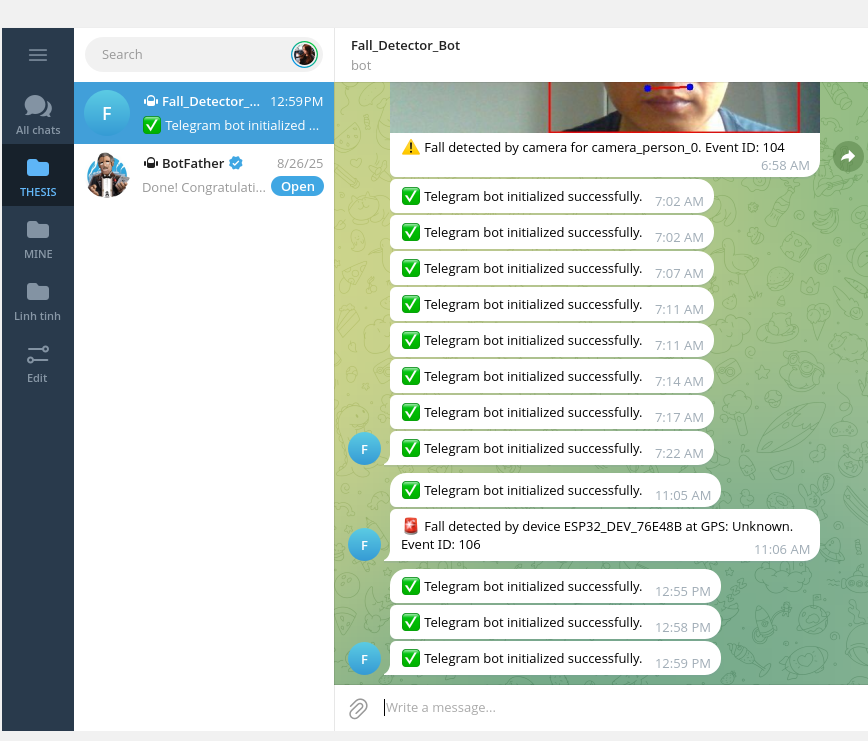
\includegraphics[width=0.8\textwidth]{figures/telegram_fall_module1_send.png}
    \caption{Thông báo cảnh báo té ngã từ module phần cứng (ESP32) qua Telegram.}
    \label{fig:telegram_hw}
\end{figure}

\begin{figure}[H]
    \centering
    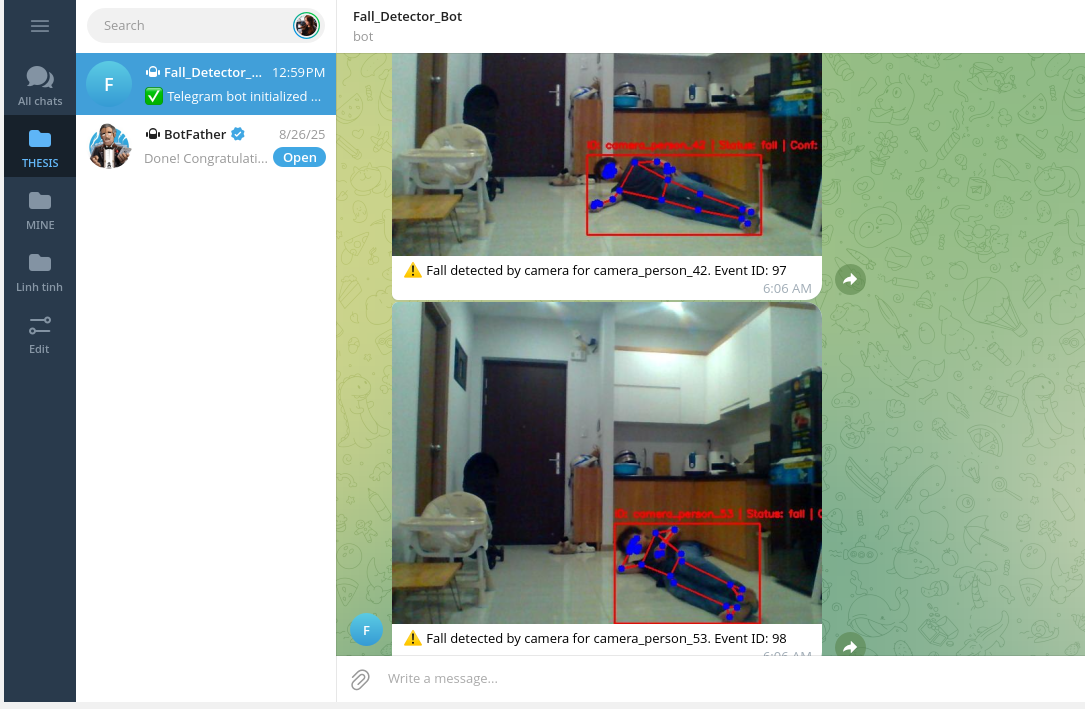
\includegraphics[width=0.8\textwidth]{figures/telegram_python_fall_send.png}
    \caption{Thông báo cảnh báo té ngã từ module xử lý hình ảnh Python qua Telegram.}
    \label{fig:telegram_python}
\end{figure}

\textit{Kết luận:} Kênh Telegram đã hoạt động ổn định, đóng vai trò cầu nối giữa hệ thống phát hiện té ngã và người dùng cuối. Việc kết hợp cả hai nguồn cảnh báo (thiết bị phần cứng và module xử lý hình ảnh) giúp tăng độ tin cậy và giảm thiểu khả năng bỏ sót sự kiện.
